% This text is proprietary.
% It's a part of presentation made by myself.
% It may not used commercial.
% The noncommercial use such as private and study is free
% Sep. 2005 
% Author: Sascha Frank 
% University Freiburg 
% www.informatik.uni-freiburg.de/~frank/
%
% additional usepackage{beamerthemeshadow} is used
%  
%  \beamersetuncovermixins{\opaqueness<1>{25}}{\opaqueness<2->{15}}
%  with this the elements which were coming soon were only hinted
\documentclass{beamer}
%\usetheme{bars}
\usepackage{beamerthemeshadow}
\begin{document}
\title{Offline Handritting Word Recognition}  
\author{Thijs Kooi, Davide Modolo}
\date{\today} 

\frame{\titlepage} 

\frame{\frametitle{Table of contents}\tableofcontents} 

% SECTION: OVERVIEW OF THE PROJECT
\section{Overview of the Project}

\frame{
\begin{beamerboxesrounded}{}
\centering Overview of the Project
\end{beamerboxesrounded}
}

\frame{\frametitle{Off-line handwriting recognition}  
\begin{itemize}
\item It involves the automatic conversion of text in an image into letter codes which are usable within computer and text-processing applications
\item Off-line handwriting recognition is comparatively difficult, as different people have different handwriting styles

\begin{figure}
  \centering
    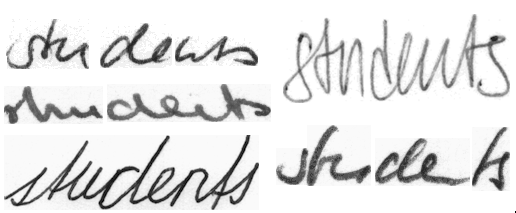
\includegraphics[width=0.5 \textwidth]{Images/studs.png}
   \caption{'Students' written by different authors}
   \label{fig:student}
\end{figure}
\end{itemize}
}

\frame{\frametitle{Our AI Project}
A lot of research has been done over the past years.\vspace{\baselineskip}

We explored the topic and implemented a full pipeline for the task.
The research touched different fields:
\begin{itemize}
\item Data Collection
\item Image Processing
\item Features extraction 
\item Machine Learning techniques
\item Word Recognition using Hidden Markov Models
\end{itemize}
}

\frame{\frametitle{Dataset}
The IAM Handwriting Database\footnote{http://www.iam.unibe.ch/fki/databases/iam-handwriting-database}
\begin{itemize}
\item It contains forms of handwritten English text which can be used to train and test handwritten text recognizers and to perform writer identification and verification experiments.
\item It contains forms of unconstrained handwritten text, which were scanned at a resolution of 300dpi and saved as PNG images with 256 gray levels. 
\item 1'539 pages of scanned text of 657 writers
\end{itemize}
}

\frame{\frametitle{Dataset}  
\begin{figure}
  \centering
    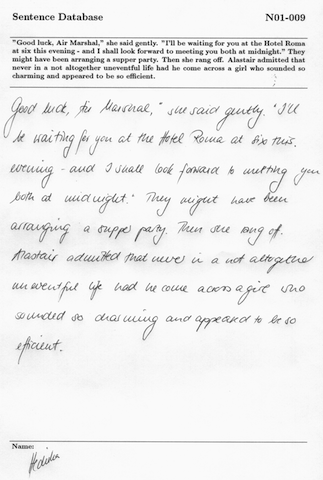
\includegraphics[width=0.5\textwidth]{Images/database.png}
   \caption{Example of page of scanned text}
   \label{fig:dataset}
\end{figure}
}


%SECTION: IMPLEMENTATION DETAILS
\section{Implementation Details}
\frame{
\begin{beamerboxesrounded}{}
\centering Implementation Details
\end{beamerboxesrounded}
}

\subsection{Pre-Process}
\frame{\frametitle{Pipeline}  
\begin{figure}
  \centering
    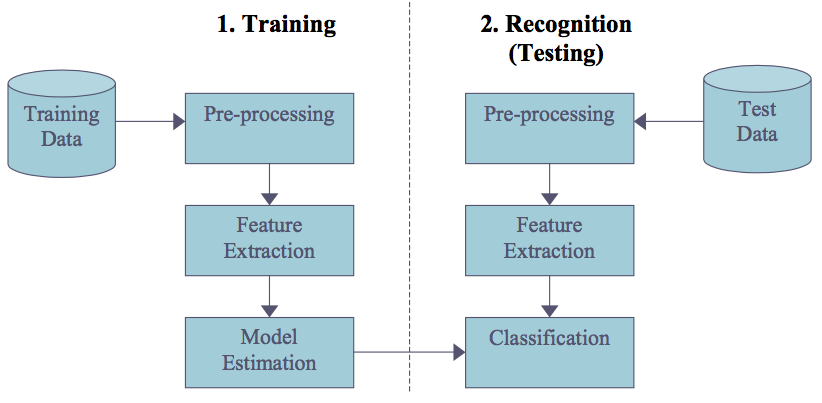
\includegraphics[width=1.02 \textwidth]{Images/pipeline.png}
   \caption{Pipeline of a word recognition system}
   \label{fig:pipeline}
\end{figure}
}


\frame{\frametitle{Line Segmentation}  
\begin{figure}
  \centering
    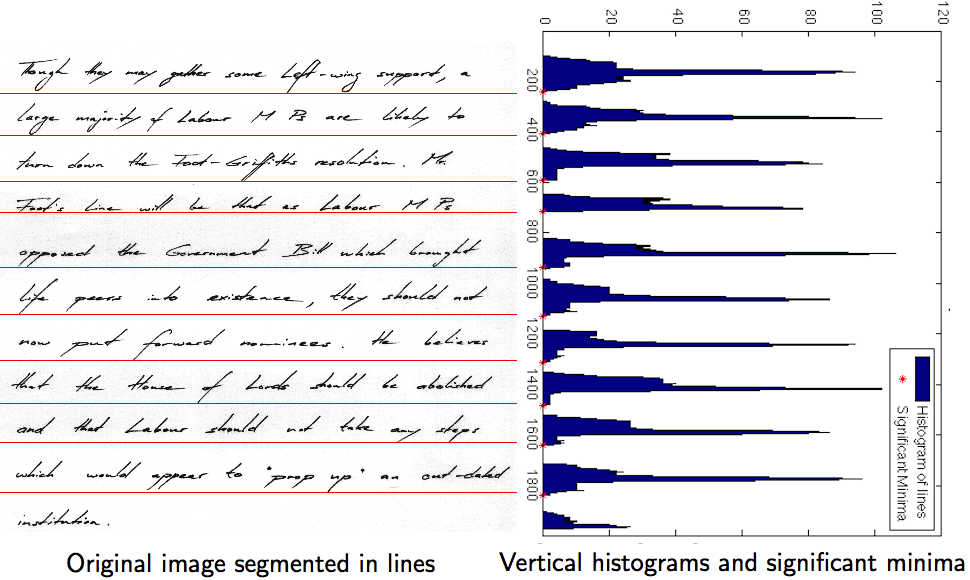
\includegraphics[width=0.96 \textwidth]{Images/line_segmentation.png}
   \caption{Example of line segmentation}
   \label{fig:lineSegm}
\end{figure}
}


\frame{\frametitle{Skew and Slope Correction}  
\begin{figure}
  \centering
    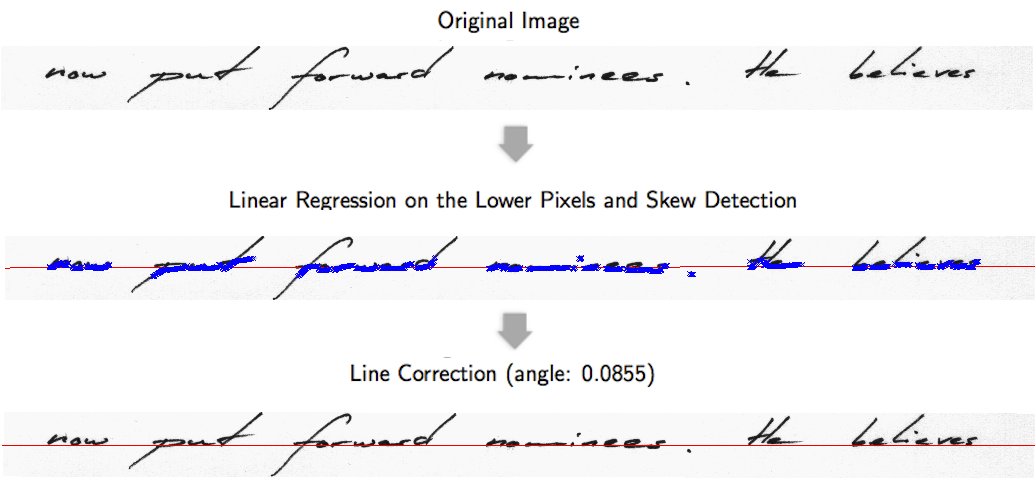
\includegraphics[width=1.0 \textwidth]{Images/skew.png}
   \caption{Skew detection and correction}
   \label{fig:skew}
\end{figure}
}


\subsection{Feature Extraction}
\frame{\frametitle{Features}  
list
}

\subsection{Hidden-Markov Model}
\frame{\frametitle{HMM}  
blabla
}


\section{Results}
\frame{\frametitle{Results}  
blabla
}



\section{Conclusions}
\frame{\frametitle{Conclusions}  
blabla
}



%\section{Pre-Processing} 
%\frame{\frametitle{Title} 
%Each frame should have a title.
%}
%
%\frame{ 
%Without title somethink is missing. 
%}
%
%
%\section{Feature Extraction} 
%\subsection{Lists I}
%\frame{\frametitle{unnumbered lists}
%\begin{itemize}
%\item Introduction to  \LaTeX  
%\item Course 2 
%\item Termpapers and presentations with \LaTeX 
%\item Beamer class
%\end{itemize} 
%}
%
%\frame{\frametitle{lists with pause}
%\begin{itemize}
%\item Introduction to  \LaTeX \pause 
%\item Course 2 \pause 
%\item Termpapers and presentations with \LaTeX \pause 
%\item Beamer class
%\end{itemize} 
%}
%
%\subsection{Lists II}
%\frame{\frametitle{numbered lists}
%\begin{enumerate}
%\item Introduction to  \LaTeX  
%\item Course 2 
%\item Termpapers and presentations with \LaTeX 
%\item Beamer class
%\end{enumerate}
%}
%\frame{\frametitle{numbered lists with pause}
%\begin{enumerate}
%\item Introduction to  \LaTeX \pause 
%\item Course 2 \pause 
%\item Termpapers and presentations with \LaTeX \pause 
%\item Beamer class
%\end{enumerate}
%}
%
%\section{Section no.3} 
%\subsection{Tables}
%\frame{\frametitle{Tables}
%\begin{tabular}{|c|c|c|}
%\hline
%\textbf{Date} & \textbf{Instructor} & \textbf{Title} \\
%\hline
%WS 04/05 & Sascha Frank & First steps with  \LaTeX  \\
%\hline
%SS 05 & Sascha Frank & \LaTeX \ Course serial \\
%\hline
%\end{tabular}}
%
%
%\frame{\frametitle{Tables with pause}
%\begin{tabular}{c c c}
%A & B & C \\ 
%\pause 
%1 & 2 & 3 \\  
%\pause 
%A & B & C \\ 
%\end{tabular} }
%
%
%\section{Section no. 4}
%\subsection{blocs}
%\frame{\frametitle{blocs}
%
%\begin{block}{title of the bloc}
%bloc text
%\end{block}
%
%\begin{exampleblock}{title of the bloc}
%bloc text
%\end{exampleblock}
%
%
%\begin{alertblock}{title of the bloc}
%bloc text
%\end{alertblock}
%}
\end{document}

